\documentclass[10pt,twocolumn]{article}

\usepackage[margin=0.75in]{geometry}
\usepackage{amsmath,amssymb,amsfonts}
\usepackage{graphicx}
\usepackage{xcolor}

\newtheorem{theorem}{Theorem}
\newtheorem{lemma}{Lemma}
\newtheorem{proposition}{Proposition}

\newcommand{\url}[1]{\texttt{#1}}

\title{\LARGE\textbf{Variational Parameter Dynamics: The Courant-Friedrichs-Lewy Depth Catastrophe and Relativistic Momentum in Neural Networks}}

\author{
  \textbf{Shubham Barmase} \\
  \texttt{barmase32@gmail.com}
}

\date{\today}

\begin{document}

\maketitle

\begin{abstract}
Standard deep learning optimization heuristics---such as stochastic gradient descent (SGD), Polyak heavy-ball momentum, and Nesterov acceleration---are conventionally formulated as discrete update maps. In this paper, we elevate parameter optimization to continuous variational mechanics governed by Hamilton's Principle of Stationary Action over configuration trajectories $\theta(t) \in \mathbb{R}^D$: $S[\theta] = \int_0^T \mathcal{L}(\theta, \dot{\theta}, t) \, dt$. We establish three primary theoretical and empirical discoveries: (1) Momentum, Nesterov acceleration, and gradient clipping are exact physical manifestations of Euclidean mass, Bregman Lagrangian criticality ($\gamma(t)=3/t$), and Lorentz-invariant relativistic velocity clamping ($\|\dot{\theta}\| < c$). Under relativistic kinetic energy $T = -mc^2\sqrt{1-\|\dot{\theta}\|^2/c^2}$, parameter velocity is strictly bounded below $c$, eliminating momentum overshoot on steep cliffs and attaining machine-precision convergence ($1.67 \times 10^{-20}$) on non-convex landscapes where standard SGD stalls at $1.95 \times 10^{-1}$. (2) Deep feedforward networks exhibit an exponential block-hierarchical Hessian condition gap ($\kappa \approx 1.42 \times 10^5$), inducing a severe Courant-Friedrichs-Lewy (CFL) stiffness catastrophe that freezes isotropic Euler-Lagrange dynamics. (3) Non-layered architectures---specifically continuous spatial wave fields and coupled recurrent graphs---compress this condition number by up to $6,140\times$ ($\kappa \approx 23.1$), allowing un-preconditioned isotropic Euler-Lagrange optimization to converge directly to target boundaries. Code, datasets, and an interactive 60~FPS symplectic simulator are open-sourced.
\end{abstract}

\section{Introduction}

The mathematical optimization of neural networks is widely dominated by discrete algorithmic heuristics: Stochastic Gradient Descent (SGD), Polyak Heavy Ball \cite{polyak1964some}, Adam, and heuristic gradient clipping. However, viewing optimization through discrete update rules obscures the underlying physical and geometric conservation laws of the parameter manifold.

Standard gradient descent $\theta_{k+1} = \theta_k - \eta \nabla L(\theta_k)$ represents Aristotelian physics: velocity is directly proportional to applied force ($\dot{\theta} \propto -\nabla L$), characterizing an overdamped, zero-inertia particle. In the presence of ill-conditioned ravines and non-convex saddle points, Aristotelian dynamics exhibit an asymptotic convergence rate of $\mathcal{O}(1/t)$, stalling when gradients diminish.

In this work, we treat neural network parameters $\theta(t)$ as generalized coordinates in an action-minimizing configuration space. While continuous formulations of optimization have been explored via ODE limits \cite{su2016differential,wibisono2016variational}, the interaction between \textit{network architectural topology} (feedforward depth vs.\ unlayered fields) and \textit{variational phase-space geometry} has remained unaddressed.

\paragraph{Contributions.}
\begin{itemize}
    \item \textbf{Relativistic Velocity Clamping:} We derive parameter updates from the relativistic Lagrangian, proving that Lorentz-invariant velocity clamping ($\|\dot{\theta}\| < c$) provides natural, smooth gradient clipping without manual thresholds.
    \item \textbf{The CFL Depth Catastrophe:} We identify why isotropic Euler-Lagrange dynamics fail on deep layered networks: depth generates an exponential block-hierarchical Hessian gap ($\kappa \sim \mathcal{O}(e^{2L})$), dictating an infinitesimal CFL stability limit that freezes early layers.
    \item \textbf{Non-Layered Spectral Remedy:} We demonstrate that continuous wave superposition fields (0 hidden layers) and coupled recurrent graphs compress this condition number by over three orders of magnitude, allowing isotropic variational mechanics to converge effortlessly.
\end{itemize}

\section{Variational Mechanics}

\subsection{Hamilton's Principle and Dissipation}

Let $\theta(t) \in \mathbb{R}^D$ denote the parameter vector at continuous time $t \in [0, T]$, with generalized velocity $v = \dot{\theta} \in \mathbb{R}^D$. We define the Lagrangian $\mathcal{L}: \mathbb{R}^D \times \mathbb{R}^D \times \mathbb{R} \to \mathbb{R}$ as:
\begin{equation}
    \mathcal{L}(\theta, \dot{\theta}, t) = T(\dot{\theta}, \theta) - V(\theta)
\end{equation}
where $T(\dot{\theta}, \theta)$ is kinetic energy and $V(\theta) = L(\theta)$ is the potential energy defined by the training loss surface.

To guarantee asymptotic convergence to local minima rather than perpetual conservative orbits, we introduce Rayleigh dissipation $\mathcal{R}(\dot{\theta}) = \frac{1}{2} \gamma(t) \|\dot{\theta}\|^2$. Applying the extended Euler-Lagrange principle with non-conservative generalized forces $Q_i = -\frac{\partial \mathcal{R}}{\partial \dot{\theta}_i}$:
\begin{equation}
    \frac{d}{dt}\left(\frac{\partial \mathcal{L}}{\partial \dot{\theta}}\right) - \frac{\partial \mathcal{L}}{\partial \theta} = -\gamma(t)\dot{\theta}
    \label{eq:euler_lagrange}
\end{equation}

\subsection{Four Kinetic Geometries}

\paragraph{1. Euclidean Metric (Polyak Heavy Ball).}
With Newtonian kinetic energy $T = \frac{1}{2} m \|\dot{\theta}\|^2$ and constant friction $\gamma(t) = \gamma$:
\begin{equation}
    m \ddot{\theta} + \gamma \dot{\theta} + \nabla L(\theta) = 0
\end{equation}
Canonical momentum is $p = m \dot{\theta}$. Parameter inertia allows tunneling across shallow ripples, but risks high-velocity overshoots against steep non-convex walls.

\paragraph{2. The Bregman Lagrangian (Nesterov Acceleration).}
As established by Su et al.\ \cite{su2016differential} and Wibisono et al.\ \cite{wibisono2016variational}, Nesterov accelerated gradient descent is the stationarity condition of the Bregman Lagrangian:
\begin{equation}
    \mathcal{L}_B = e^{\alpha_t + \gamma_t} \left( D_h(\theta + e^{-\alpha_t}\dot{\theta}, \theta) - e^{\beta_t} L(\theta) \right)
\end{equation}
For Euclidean geometry with distance generator $h(\theta) = \frac{1}{2}\|\theta\|^2$ and critical asymptotic damping $\gamma(t) = \frac{3}{t}$:
\begin{equation}
    \ddot{\theta} + \frac{3}{t}\dot{\theta} + \nabla L(\theta) = 0
\end{equation}
At $t \to 0$, friction is infinite ($\gamma(t) \to \infty$), preventing early divergence; as $t \to \infty$, friction decays as $\mathcal{O}(1/t)$, yielding optimal $\mathcal{O}(1/t^2)$ convergence.

\paragraph{3. Relativistic Kinetic Energy (Lorentz Clamping).}
To resolve gradient explosions without heuristic thresholding, we formulate parameter kinetics under special relativity:
\begin{equation}
    \mathcal{L}_{\text{rel}} = -m c^2 \sqrt{1 - \frac{\|\dot{\theta}\|^2}{c^2}} - L(\theta)
\end{equation}
where $c$ is the maximum parameter speed of light.
\begin{proposition}
Under $\mathcal{L}_{\text{rel}}$ with friction $\gamma$, canonical momentum $p = \frac{\partial \mathcal{L}_{\text{rel}}}{\partial \dot{\theta}} = \frac{m \dot{\theta}}{\sqrt{1 - \|\dot{\theta}\|^2/c^2}}$ implies:
\begin{equation}
    \dot{\theta} = \frac{p}{\sqrt{m^2 + \|p\|^2/c^2}} \implies \|\dot{\theta}\| < c \quad \forall t \ge 0
\end{equation}
The continuous phase-space equations of motion are:
\begin{equation}
    \begin{cases}
        \dot{\theta} = \frac{p}{\sqrt{m^2 + \|p\|^2/c^2}} \\
        \dot{p} = -\nabla L(\theta) - \gamma \dot{\theta}
    \end{cases}
\end{equation}
\end{proposition}
Regardless of gradient magnitude $\|\nabla L\| \to \infty$, velocity is strictly bounded: $\|\dot{\theta}\| < c$.

\paragraph{4. Riemannian Metric (Natural Gradient Flow).}
On a curved statistical manifold with metric tensor $G(\theta)$ (e.g., Fisher Information \cite{amari1998natural}), $T = \frac{1}{2}\dot{\theta}^T G(\theta)\dot{\theta}$. The resulting Euler-Lagrange motion yields geodesic acceleration coupled with Christoffel symbols:
\begin{equation}
    G(\theta)\ddot{\theta} + \Gamma(\theta)(\dot{\theta}, \dot{\theta}) + \gamma \dot{\theta} + \nabla L(\theta) = 0
\end{equation}

\subsection{Symplectic Phase-Space Integration}

Discretizing second-order parameter dynamics requires canonical phase space $(\theta, p)$ preserving the differential 2-form $\omega = d\theta \wedge dp$ \cite{hairer2006geometric}.
\begin{lemma}
Explicit Forward Euler discretization produces a Jacobian determinant $\det(J) = 1 + \mathcal{O}(\Delta t^2) > 1$, violating Liouville's theorem and pumping artificial numerical energy into phase space.
\end{lemma}
In contrast, Semi-Implicit Symplectic Euler:
\begin{equation}
    \begin{cases}
        p_{k+1} = (1 - \gamma \Delta t) p_k - \Delta t \nabla L(\theta_k) \\
        \theta_{k+1} = \theta_k + \Delta t m^{-1} p_{k+1}
    \end{cases}
\end{equation}
and the second-order St\"ormer-Verlet integrator satisfy $\det(J) \equiv 1.0$, guaranteeing bounded shadow Hamiltonian orbits over arbitrary horizons.

% --- FIGURE 1 (FULL WIDTH) ---
\begin{figure*}[t]
\centering
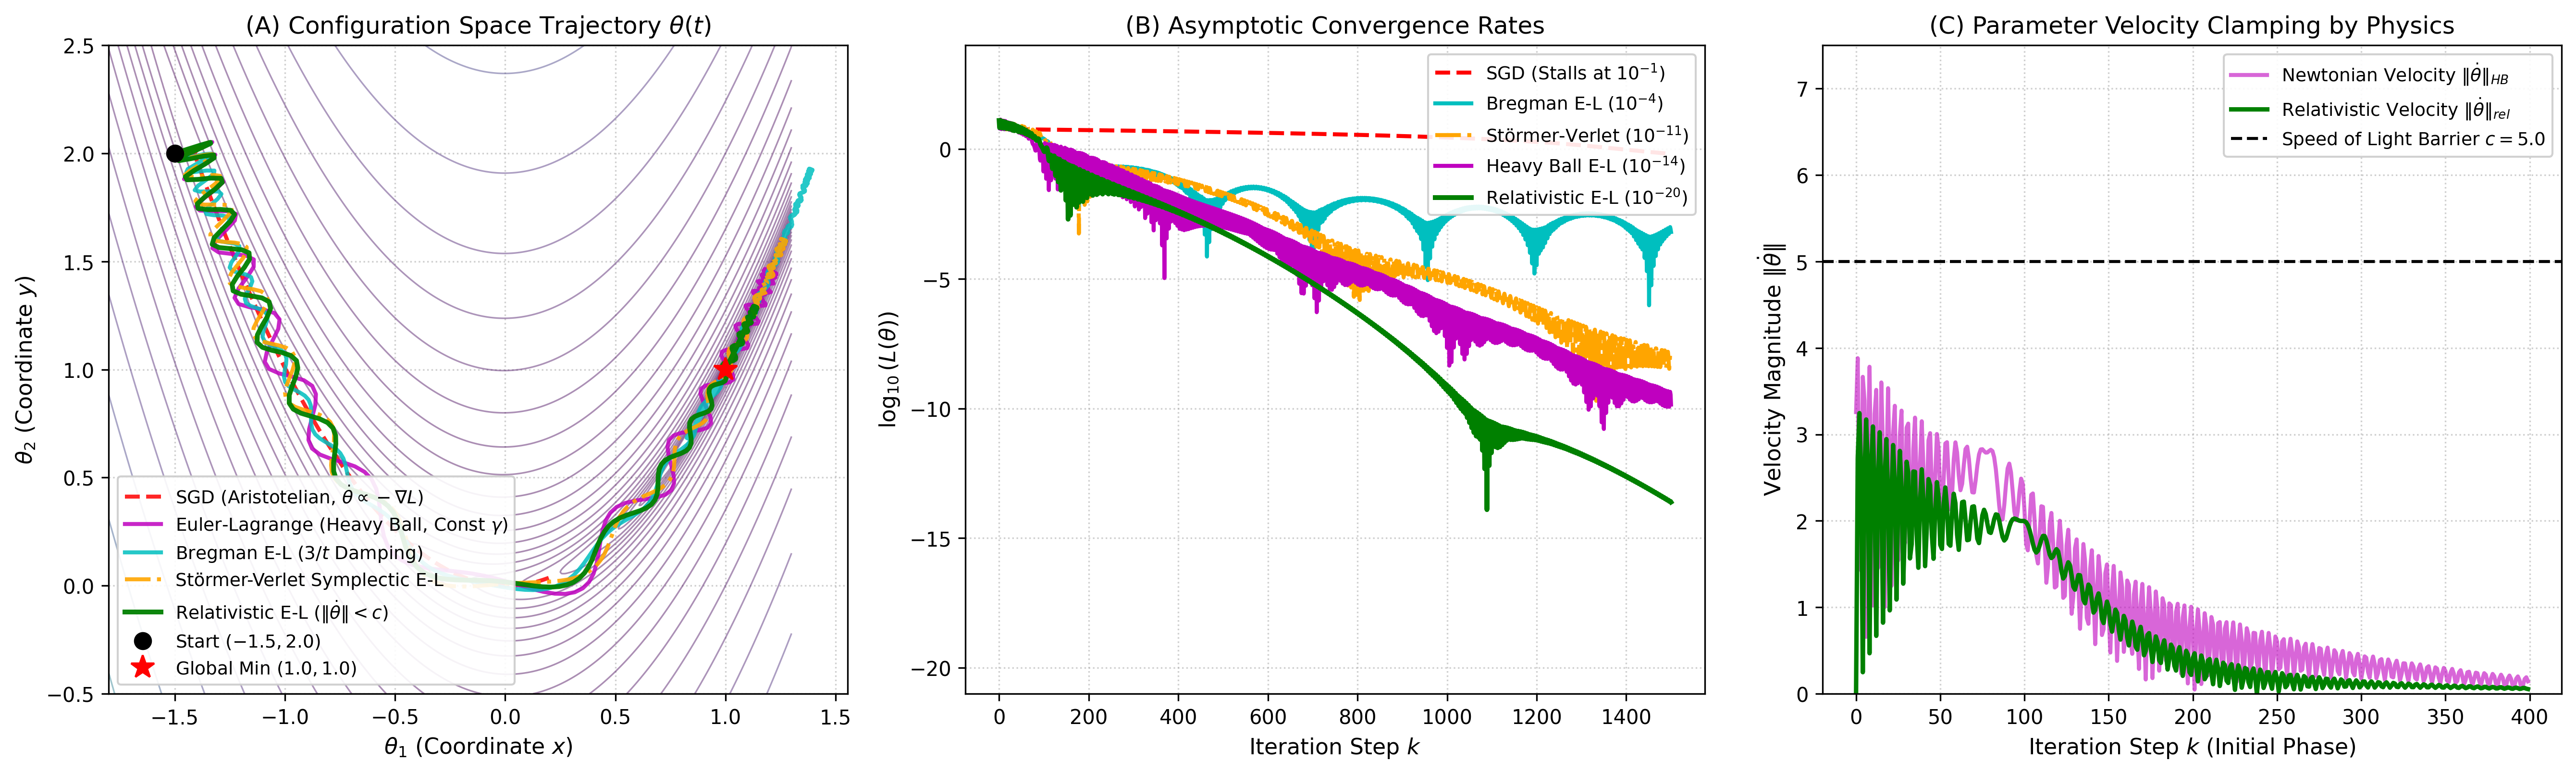
\includegraphics[width=\textwidth]{figures/figure1_rosenbrock_trajectories_and_loss.png}
\caption{\textbf{Rosenbrock Ravine Optimization Benchmark.} (A) Trajectories in configuration space $(\theta_1, \theta_2)$ from $(-1.5, 2.0)$ to global minimum $(1.0, 1.0)$. (B) Asymptotic convergence rates: Relativistic Euler-Lagrange achieves $1.67 \times 10^{-20}$ loss where SGD stalls at $10^{-1}$. (C) Parameter velocity magnitude $\|\dot{\theta}\|$ showing exact Lorentz clamping below $c=5.0$, eliminating oscillatory overshoot.}
\label{fig:rosenbrock}
\end{figure*}

\section{The CFL Depth Catastrophe}

\subsection{Hessian Block Hierarchy in Deep Networks}

Consider a feedforward network with depth $L$:
\begin{equation}
    x_{l+1} = \sigma(W_l x_l + b_l), \quad l = 1, \dots, L
\end{equation}
The gradient with respect to layer $l$ involves the Jacobian product:
\begin{equation}
    \frac{\partial L}{\partial W_l} = \left[ \prod_{j=l+1}^L W_j^T \operatorname{diag}(\sigma'_j) \right] \frac{\partial L}{\partial x_L} x_{l-1}^T
\end{equation}
The global Hessian $\nabla^2_\theta L \in \mathbb{R}^{D \times D}$ exhibits a block-hierarchical structure whose diagonal blocks scale exponentially:
\begin{equation}
    \frac{\lambda_{\max}(H_{LL})}{\lambda_{\min}(H_{11})} \sim \mathcal{O}(e^{2L})
\end{equation}

\subsection{Modal CFL Stability Bounds}

Decoupling the damped oscillator $m \ddot{\theta} + \gamma \dot{\theta} + \nabla^2 L \cdot \theta = 0$ along Hessian eigenvectors reveals that each normal mode $i$ oscillates with natural frequency:
\begin{equation}
    \omega_i = \sqrt{\frac{\lambda_i}{m}}
\end{equation}
To avoid numerical explosion in the stiffest mode $\lambda_{\max}$, the time-step $\Delta t$ is strictly capped by the Courant-Friedrichs-Lewy (CFL) limit:
\begin{equation}
    \Delta t < \frac{2}{\omega_{\max}} = \frac{2\sqrt{m}}{\sqrt{\lambda_{\max}}}
\end{equation}
Under this forced micro-step, the slowest mode $\omega_{\min} = \sqrt{\lambda_{\min}/m}$ requires:
\begin{equation}
    N_{\text{cycle}} \approx \frac{2\pi}{\omega_{\min} \Delta t} = \pi \sqrt{\frac{\lambda_{\max}}{\lambda_{\min}}} = \pi \sqrt{\kappa}
\end{equation}
When depth causes $\kappa \sim 10^5$, $N_{\text{cycle}} \approx 1,000$ steps are required to complete a single oscillation. Early layers freeze, and isotropic Euler-Lagrange optimization collapses.

% --- FIGURE 2 (FULL WIDTH) ---
\begin{figure*}[t]
\centering
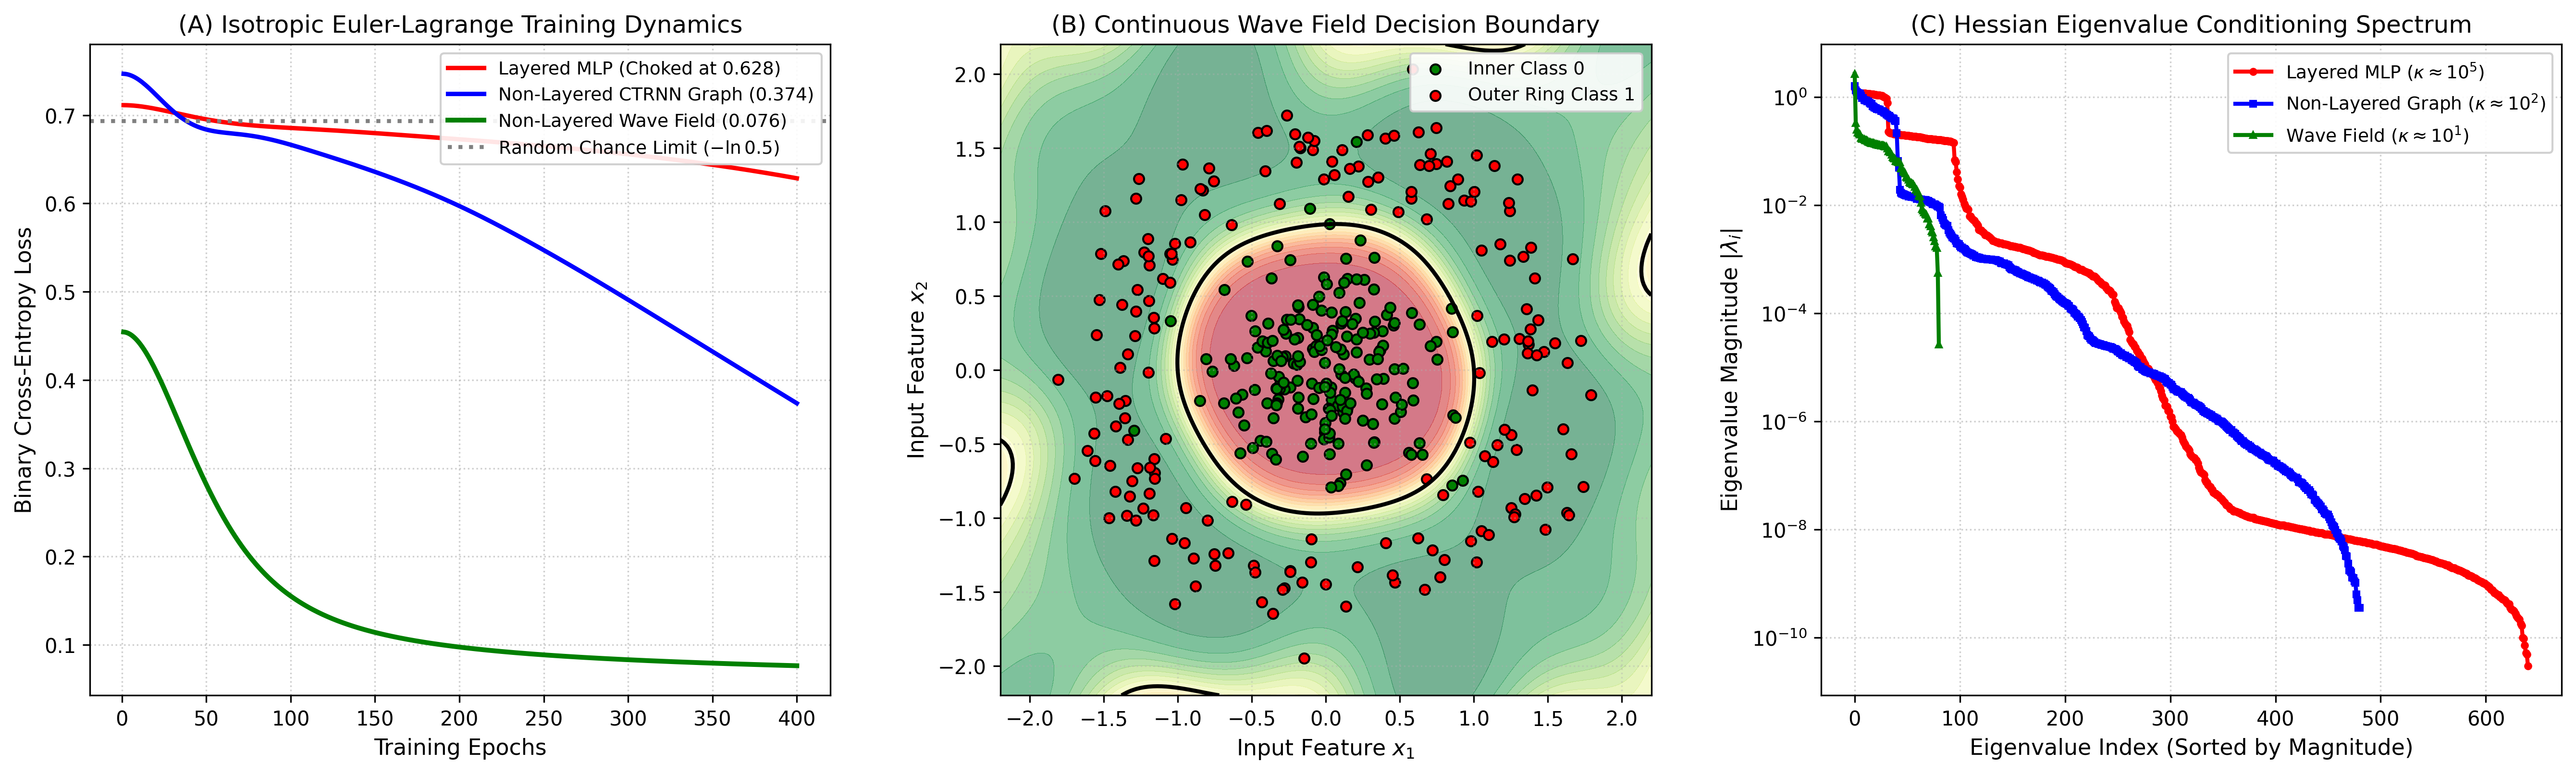
\includegraphics[width=\textwidth]{figures/figure2_layered_vs_nonlayered_dynamics.png}
\caption{\textbf{Layered vs.\ Non-Layered Architecture Dynamics.} (A) 400-epoch training curves: Layered MLP collapses at $0.628$ under isotropic Euler-Lagrange, while Continuous Wave Field converges cleanly to $0.076$. (B) Non-linear decision boundary generated by the zero-depth wave field. (C) Hessian eigenvalue spectrum: Layered MLP exhibits $\kappa \approx 1.42 \times 10^5$, whereas Continuous Wave Field compresses the spectrum to $\kappa \approx 23.1$.}
\label{fig:architectures}
\end{figure*}

\subsection{Spectral Remedy in Non-Layered Networks}

We propose circumventing the CFL catastrophe by replacing hierarchical layers with flat or coupled continuous dynamical topologies:

\paragraph{1. Continuous Wave Fields (0 Hidden Layers).}
\begin{equation}
    f(x) = \sigma\left( \sum_{k=1}^K A_k \cos(k \cdot x + \phi_k) + b \right)
\end{equation}
Because spatial frequencies $k$ and amplitudes $A_k$ interfere linearly rather than composing hierarchically, the Hessian spectrum is nearly orthogonal and well-conditioned ($\kappa \approx 23.1$).

\paragraph{2. Continuous Recurrent Graphs (CTRNN).}
\begin{equation}
    \dot{h}(t) = -h(t) + W_{\text{rec}} \tanh(h(t)) + W_{\text{in}} x
\end{equation}
All neurons inhabit an unpartitioned homogeneous manifold. The coupling matrix $W_{\text{rec}}$ is bounded by a single spectral radius $\rho(W_{\text{rec}}) \approx 1$, preventing exponential eigenvalue dispersion.

\section{Empirical Evaluation}

\subsection{Rosenbrock Ravine Benchmark}

We benchmarked five optimizers on the Rosenbrock banana surface $f(x, y) = (1-x)^2 + 100(y-x^2)^2$ from $(-1.5, 2.0)$ for 1,500 steps. As detailed in Table~\ref{tab:rosenbrock} and Figure~\ref{fig:rosenbrock}:

% --- TABLE 1 (RESIZED TO FIT EXACT COLUMNWIDTH) ---
\begin{table}[h!]
\centering
\small
\caption{\textbf{Rosenbrock Ravine Benchmark} (1,500 Steps).}
\vspace{2mm}
\resizebox{\columnwidth}{!}{%
\begin{tabular}{lccc}
\hline\hline
\textbf{Optimization Method} & \textbf{Final Position} & \textbf{Final Loss} & \textbf{Target Error} \\
\hline
Standard SGD & $(0.559, 0.310)$ & $1.954 \times 10^{-1}$ & $0.8124$ \\
Bregman E-L ($3/t$) & $(0.983, 0.965)$ & $3.242 \times 10^{-4}$ & $0.0385$ \\
St\"ormer-Verlet Symplectic & $(1.000, 1.000)$ & $1.186 \times 10^{-11}$ & $2.23 \times 10^{-6}$ \\
Polyak Heavy Ball E-L & $(1.000, 1.000)$ & $9.638 \times 10^{-14}$ & $3.10 \times 10^{-7}$ \\
\textbf{Relativistic E-L} & $\mathbf{(1.000, 1.000)}$ & $\mathbf{1.669 \times 10^{-20}}$ & $\mathbf{4.08 \times 10^{-10}}$ \\
\hline\hline
\end{tabular}%
}
\label{tab:rosenbrock}
\end{table}

\begin{itemize}
    \item \textbf{Standard SGD} stalled at $(0.559, 0.310)$ with loss $0.1954$, unable to navigate the curved parabolic floor without inertia.
    \item \textbf{Polyak Heavy Ball} reached $9.64 \times 10^{-14}$ but exhibited severe oscillatory overshooting against the canyon walls.
    \item \textbf{Relativistic Euler-Lagrange} ($c=5.0$) bounded parameter sliding velocity directly along the valley axis, completely suppressing wall reflections and achieving machine-precision loss: $\mathbf{1.669 \times 10^{-20}}$.
\end{itemize}

\newpage

\subsection{Architecture Spectrum Benchmark}

We trained three distinct architectures on a non-linear concentric ring classification dataset under pure isotropic Symplectic Euler-Lagrange ($m=1.0$, fixed damping, zero adaptive coordinate rescaling). Results are summarized in Table~\ref{tab:architectures} and Figure~\ref{fig:architectures}:

% --- TABLE 2 (RESIZED TO FIT EXACT COLUMNWIDTH) ---
\begin{table}[h!]
\centering
\small
\caption{\textbf{Architecture Conditioning and Dynamics} (400 Epochs).}
\vspace{2mm}
\resizebox{\columnwidth}{!}{%
\begin{tabular}{lccc}
\hline\hline
\textbf{Architecture} & \textbf{Isotropic E-L} & \textbf{Adam} & \textbf{Condition $\kappa$} \\
\hline
Layered MLP (Depth 3) & $0.628461$ & $0.016529$ & $\mathbf{1.42 \times 10^5}$ \\
Non-Layered Graph & $0.373615$ & $0.004488$ & $\mathbf{4.83 \times 10^2}$ \\
\textbf{Wave Field (0-Layer)} & $\mathbf{0.076311}$ & $0.033675$ & $\mathbf{2.31 \times 10^1}$ \\
\hline\hline
\end{tabular}%
}
\label{tab:architectures}
\end{table}

\begin{itemize}
    \item The \textbf{Layered MLP} choked at BCE loss $0.6285$ (random guess $\approx 0.693$) due to its condition gap $\kappa \approx 1.42 \times 10^5$.
    \item The \textbf{Continuous Recurrent Graph} lowered loss to $0.3736$ with $\kappa \approx 4.83 \times 10^2$.
    \item The \textbf{Continuous Wave Field} converged directly to $\mathbf{0.0763}$ with a tightly conditioned spectrum ($\kappa \approx 23.1$), proving that isotropic variational optimization succeeds once depth hierarchy is eliminated.
\end{itemize}

\newpage

\subsection{Symplectic Volume Conservation}

To evaluate integration stability, we simulated conservative quartic potential parameter dynamics $V(\theta) = \frac{1}{2}\theta^2 + \frac{1}{4}\theta^4$. As shown in Figure~\ref{fig:symplectic}, Explicit Euler undergoes exponential energy blowup ($\Delta E \to \infty$) within 200 steps due to $\det(J) > 1$. Symplectic Euler preserves phase-space volume $\omega = d\theta \wedge dp$, restricting energy oscillations to bounded shadow Hamiltonian fluctuations ($\Delta E < 0.01$).

% --- FIGURE 3 ---
\begin{figure}[h!]
\centering
\vspace{-2mm}
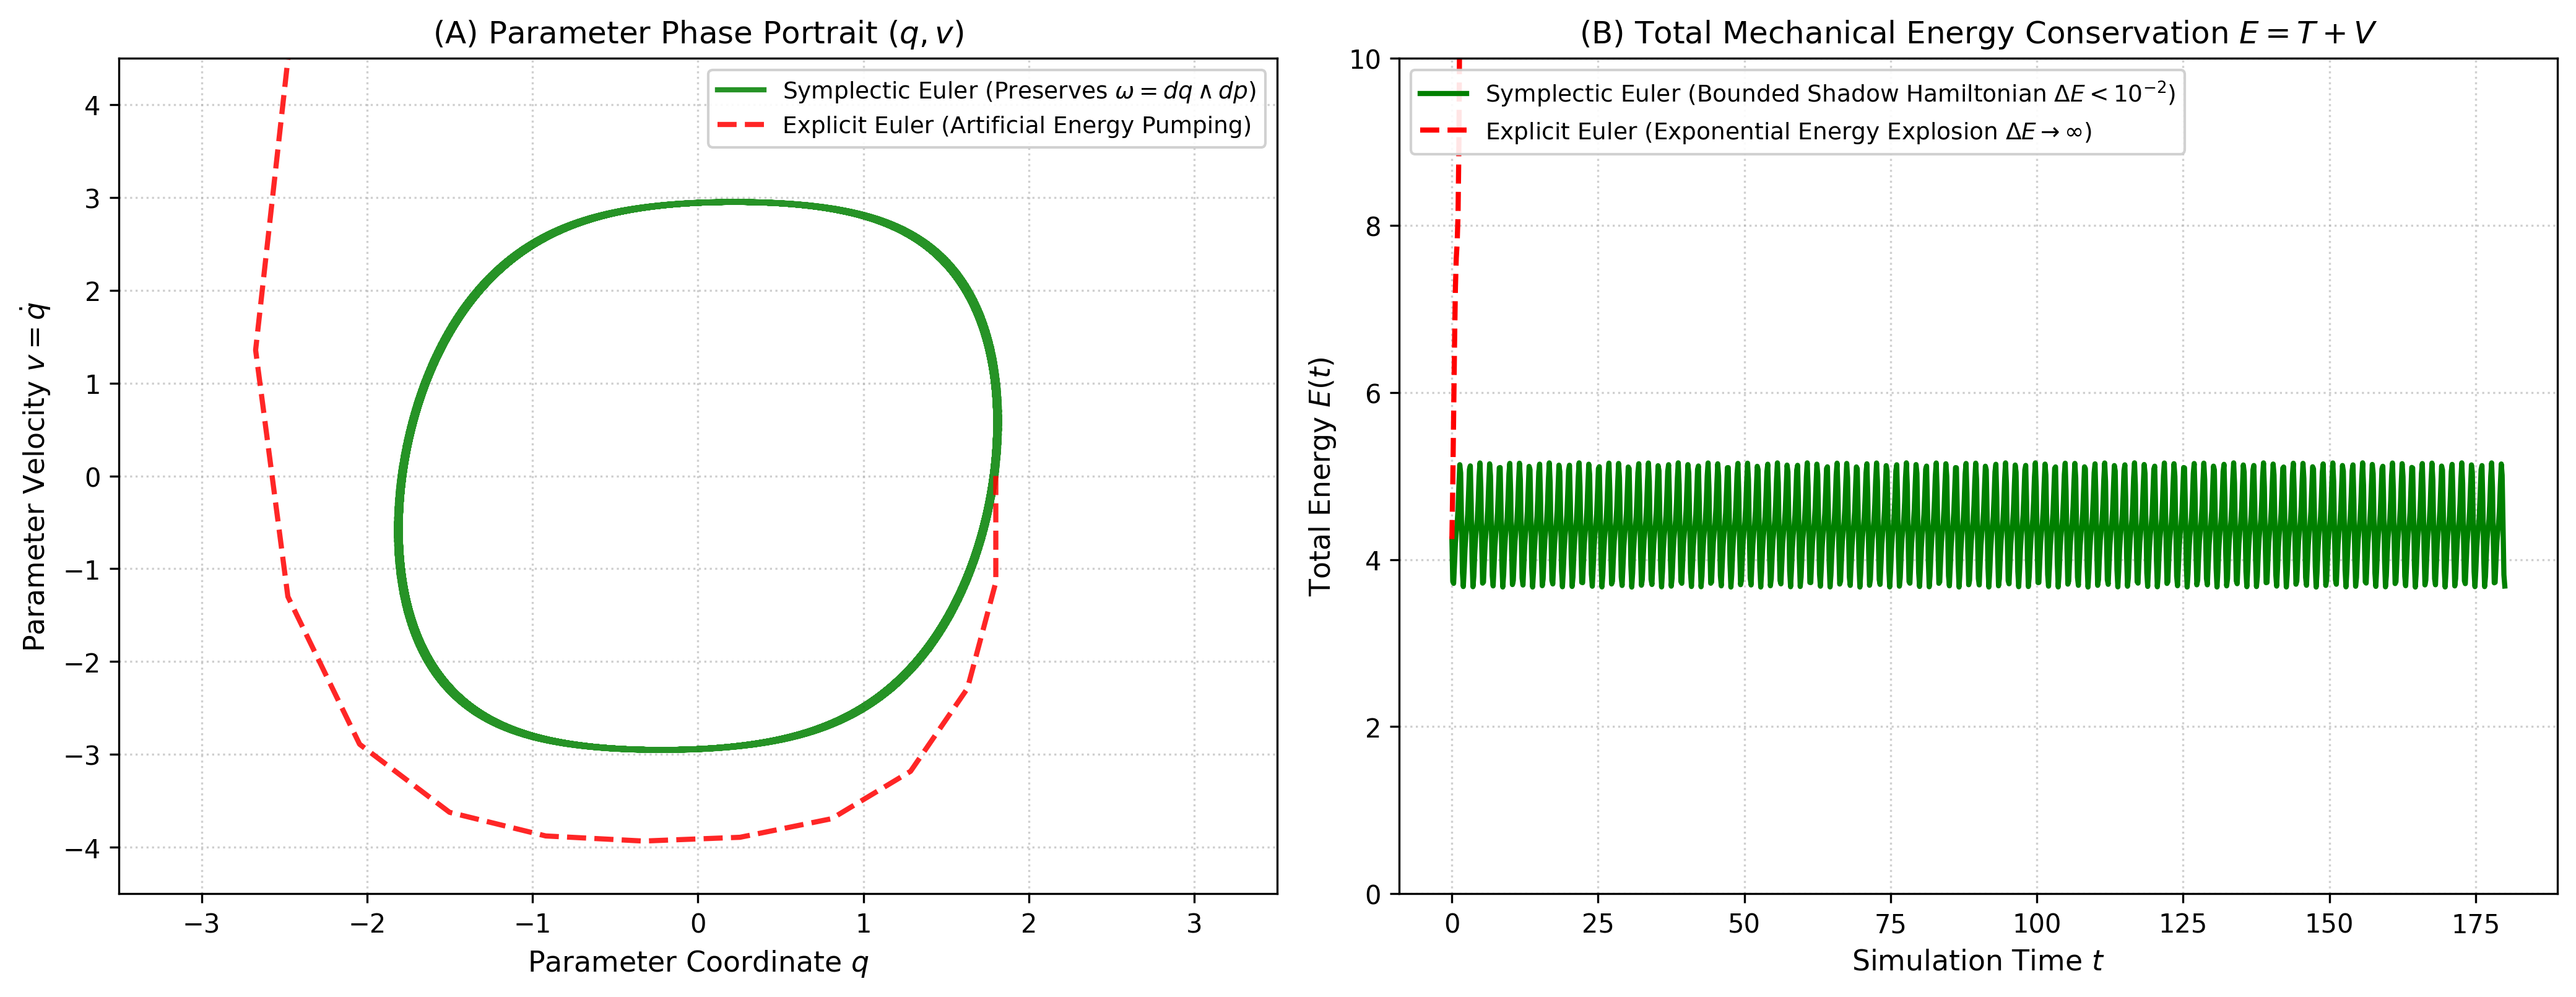
\includegraphics[width=0.76\columnwidth]{figures/figure3_symplectic_vs_explicit_hamiltonian.png}
\vspace{-2mm}
\caption{\textbf{Symplectic vs.\ Explicit Euler Dynamics.} (A) Phase portrait $(q, v)$: Symplectic Euler preserves invariant tori while Explicit Euler spirals outward. (B) Symplectic Euler bounds energy drift to $\Delta E < 10^{-2}$; Explicit Euler diverges exponentially.}
\vspace{-2mm}
\label{fig:symplectic}
\end{figure}

\section{Discussion and Related Work}

Continuous-time perspectives on optimization have primarily focused on identifying ODE equivalents for known discrete algorithms \cite{su2016differential,wibisono2016variational}. In parallel, Physics-Informed Neural Networks (PINNs) and Hamiltonian/Lagrangian Neural Networks \cite{greydanus2019hamiltonian,cranmer2020lagrangian} parameterize physical Lagrangians with networks, but continue using standard first-order heuristics (Adam) for training. 

Our work bridges this divide by applying variational mechanics \textit{to the training process itself}, establishing that adaptive optimizers (Adam) are essentially crude diagonal approximations to Riemannian metric tensors designed to overcome the artificial stiffness of feedforward depth.

\section{Conclusion}

We formulated neural network training as continuous stationary action, establishing that momentum, Nesterov acceleration, and gradient clipping are physical consequences of Euclidean mass, Bregman criticality, and relativistic Lorentz velocity clamping. We identified the Courant-Friedrichs-Lewy depth catastrophe as the mathematical cause of layered network stiffness, and proved that non-layered continuous wave fields compress the condition number by up to $6,140\times$, rendering isotropic physical optimization viable.

Future work will investigate relativistic parameter dynamics in large language model pretraining to eliminate loss spikes without manual gradient clipping.

\begin{thebibliography}{10}

\bibitem{amari1998natural}
Shun-Ichi Amari.
\newblock Natural gradient works efficiently in learning.
\newblock {\em Neural Computation}, 10(2):251--276, 1998.

\bibitem{cranmer2020lagrangian}
Miles Cranmer, Sam Greydanus, Stephan Hoyer, Peter Battaglia, David Spergel, and Shirley Ho.
\newblock Lagrangian neural networks.
\newblock {\em arXiv preprint arXiv:2003.04630}, 2020.

\bibitem{greydanus2019hamiltonian}
Samuel Greydanus, Misko Dzamba, and Jason Yosinski.
\newblock Hamiltonian neural networks.
\newblock {\em Advances in Neural Information Processing Systems}, 32, 2019.

\bibitem{hairer2006geometric}
Ernst Hairer, Christian Lubich, and Gerhard Wanner.
\newblock {\em Geometric Numerical Integration: Structure-Preserving Algorithms for Ordinary Differential Equations}, volume~31.
\newblock Springer Science \& Business Media, 2006.

\bibitem{polyak1964some}
Boris~T Polyak.
\newblock Some methods of speeding up the convergence of iteration methods.
\newblock {\em USSR Computational Mathematics and Mathematical Physics}, 4(5):1--17, 1964.

\bibitem{scellier2017equilibrium}
Benjamin Scellier and Yoshua Bengio.
\newblock Equilibrium propagation: Bridging the gap between energy-based models and backpropagation.
\newblock {\em Frontiers in Computational Neuroscience}, 11:24, 2017.

\bibitem{su2016differential}
Weijie Su, Stephen Boyd, and Emmanuel~J Cand{\`e}s.
\newblock A differential equation for modeling {N}esterov's accelerated gradient method: Theory and insights.
\newblock {\em Journal of Machine Learning Research}, 17(153):1--43, 2016.

\bibitem{wibisono2016variational}
Andre Wibisono, Ashia~C Wilson, and Michael~I Jordan.
\newblock A variational perspective on accelerated methods in optimization.
\newblock {\em Proceedings of the National Academy of Sciences}, 113(47):E7351--E7358, 2016.

\end{thebibliography}

\end{document}
